\newpage
\section{Qualità di processo}

	Per garantire la qualità del prodotto finale è necessario garantire la qualità dei processi necessari al suo completamento. A questo scopo, si è deciso di adottare lo standard \textit{ISO/IEC 15504\ped{G}}, denominato \textit{SPICE\ped{G}}.
	Esso si fonda sul principio che ogni processo deve essere controllato costantemente, in modo tale da rilevare possibili errori o debolezze, e correggerli prima che essi si diffondano, provocando un aumento del carico di lavoro e dello spreco di risorse.
	\textit{SPICE\ped{G}} definisce sei livelli di maturità del processo:
	
	\begin{itemize}
		\item \textbf{Level 0 - Incomplete:} processo non ancora implementato o incapace di raggiungere i suoi obiettivi;
		\item \textbf{Level 1 - Performed:} processo messo in atto e capace di raggiungere i suoi obiettivi;
		\item \textbf{Level 2 - Managed:} processo eseguito sulla base di obiettivi ben definiti;
		\item \textbf{Level 3 - Established:} processo eseguito in base ai principi dell’ingegneria del software; 
		\item \textbf{Level 4 - Predictable:} processo attuato all’interno di limiti ben definiti;
		\item \textbf{Level 5 - Optimizing:} processo predicibile e capace di adattarsi per raggiungere obiettivi specifici e rilevanti;
	\end{itemize}
	
	Al fine di perseguire correttamente questo modello, è necessario adottare il principio \textit{PDCA\ped{G}}, il quale si compone delle seguenti quattro fasi:
	
	\begin{itemize}
		\item \textbf{Plan:} fase di pianificazione ed individuazione di obiettivi e processi necessari allo scopo di raggiungere i risultati attesi;
		\item \textbf{Do:} fase di attuazione delle attività pianificate nella precedente fase e raccolta di dati sulla qualità ottenuta;
		\item \textbf{Check:} fase di verifica dove vengono confrontati i dati in uscita dalla fase Do con quelli pianificati nella fase Plan;
		\item \textbf{Act:} fase in cui si determinano le cause delle differenze fra risultati ottenuti e risultati attesi, in modo da individuare le azioni correttive da effettuare per ottenere un miglioramento della qualità.
	\end{itemize}

	\begin{figure}[H]
		\centering
		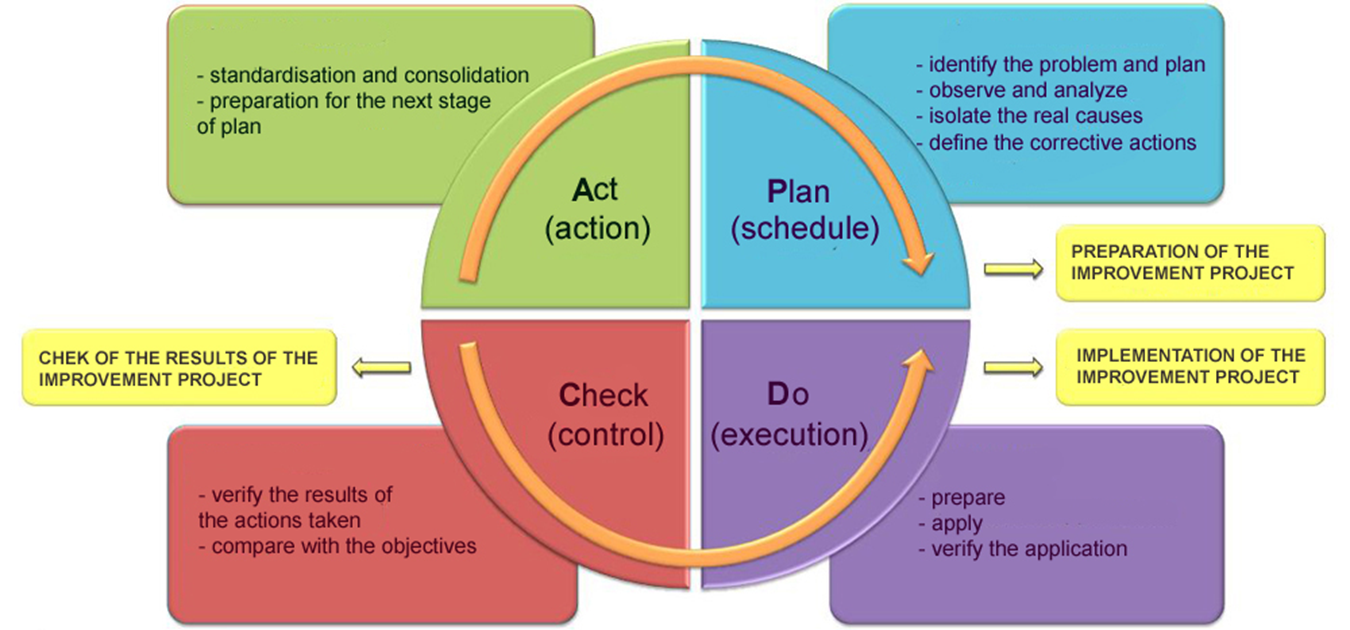
\includegraphics[scale=0.6]{includes/img/pdca.png}
		\caption{Fasi del principio PDCA.}
	\end{figure}

	Infine, il \textit{team\ped{G}} ha individuato dallo standard \textit{ISO/IEC 12207:2008\ped{G}} i processi che ritiene più importanti durante tutto il ciclo di vita del prodotto, al fine di garantire una buona qualità di processo. Per ognuno di essi sono stati individuati obiettivi e metriche coerenti con i livelli di qualità perseguiti.
	
	\subsection{Infrastructure Management Process}
	Questo processo ha lo scopo di fornire, mantenere ed aggiornare l’infrastruttura ed i servizi necessari alla realizzazione del progetto, durante tutto il suo ciclo di vita. Il termine infrastruttura comprende: elementi hardware, software, metodi, strumenti, tecniche e standard impiegati nello sviluppo del prodotto.
	L’infrastruttura necessaria allo svolgimento del progetto dovrà essere mantenuta costantemente
	aggiornata; in particolare l’utilizzo delle metriche sotto indicate permetterà l’individuazione di
	eventuali errori all’interno degli strumenti utilizzati, la cui correzione permetterà di ripristinare
	l’erogazione di dati corretti e coerenti.
		\subsubsection{Obiettivi}
		Per tutta la durata del progetto, l’infrastruttura impiegata nello sviluppo dovrà raggiungere i seguenti obiettivi:
		\begin{itemize}
			\item ogni procedura riguardante le attività svolte più frequentemente durante lo sviluppo del
			progetto, sarà descritta nel documento \textsc{NormeDiProgetto 1\_0\_0.pdf};
			\item ogni riferimento normativo ed informativo sarà completo di informazioni utili al proprio
			reperimento;
			\item la piattaforma NetBreakDB sarà a disposizione di ogni componente del team, in caso di bisogno di accesso ai dati in essa contenuti;
		\end{itemize}
		\subsubsection{Metriche}
			\paragraph{Disponibilità NetBreakDB}
			Indica la percentuale di disponibilità di utilizzo della piattaforma NetBreakDB, rispetto alle richieste di accesso.
			\begin{table}[H]
				\begin{center}
					\begin{tabular}{|c|c|c|}
						\hline
						\textbf{Metodo di calcolo} & \textbf{Range accettazione} & \textbf{Range ottimale} \\
						\hline
						n° acc corr	a pag login/n° tot richieste acc pag login inoltrate & 80-100  & 90-100 \\
						\hline
					\end{tabular}
				\end{center}
				\caption{Disponibilità NetBreakDB}
			\end{table}
	
	\subsection{Project Planning, Assessment \& Control Process}
	Questo processo ha lo scopo di produrre dei piani di sviluppo per il progetto, che comprendano:
	\begin{itemize}
		\item la scelta del modello di ciclo di vita del prodotto;
		\item le descrizioni delle attività e dei compiti da svolgere;
		\item la pianificazione temporale del lavoro e dei costi da sostenere;
		\item l'allocazione di compiti e responsabilità;
		\item le misurazioni per rilevare lo stato del progetto, rispetto alle pianificazioni stilate.
	\end{itemize}
	La pianificazione effettuata dovrà essere aggiornata costantemente durante tutta l’attività di
	progetto per essere sempre coerente con la situazione corrente. Qualsiasi eventuale valore negativo
	a livello di Schedule Variance o Budget Variance rilevato in una fase di lavoro dovrà essere
	assolutamente compensato entro la fine dell’attività di progetto, in quanto non è assolutamente
	ammesso eccedere le ore di lavoro finali e il preventivo dei costi finale indicato nella pianificazione.
		\subsubsection{Obiettivi}
		L’intero sviluppo del progetto dovrà seguire la pianificazione prodotta:
		\begin{itemize}
			\item ogni componente dovrà svolgere e portare a termine l'attività a lui assegnata, svolgendo tutti i compiti nei quali è stata suddivisa e facendo attenzione a rispettare le scadenze fissate;
			\item il costo necessario allo svolgimento di un'attività non dovrà eccedere la somma
			preventivata.
		\end{itemize}
		\subsubsection{Metriche}
			\paragraph{Schedule Variance}
			Indica se si è o meno in linea con la pianificazione temporale delle attività nella baseline.
			Se si ottiene un valore positivo significa che il team è in anticipo rispetto alla pianificazione presentata nel documento \textsc{PianoDiProgetto 1\_0\_0.pdf}, altrimenti significa che si è in ritardo.
			\begin{table}[H]
				\begin{center}
					\begin{tabular}{|c|c|c|}
						\hline
						\textbf{Metodo di calcolo} & \textbf{Range accettazione} & \textbf{Range ottimale} \\
						\hline
						att compl effett - att che dovrebbero esssere compl secondo pianific  & >=0  & >0 \\
						\hline
					\end{tabular}
				\end{center}
				\caption{Schedule Variance}
			\end{table}
		
		\paragraph{Budget Variance}
		Indica se la spesa sostenuta alla data corrente è superiore o inferiore a quella preventivata in sede di pianificazione.
		Un valore positivo indica che si è speso meno di quanto inizialmente previsto, altrimenti significa che si è speso più del preventivo.
		\begin{table}[H]
			\begin{center}
				\begin{tabular}{|c|c|c|}
					\hline
					\textbf{Metodo di calcolo} & \textbf{Range accettazione} & \textbf{Range ottimale} \\
					\hline
					costo pianif per realiz att di progetto alla data corr - costo effett sost alla data corr & >=0  & >0 \\
					\hline
				\end{tabular}
			\end{center}
			\caption{Budget Variance}
		\end{table}
	
	\subsection{Risk Management Process}
	Questo processo ha l'obiettivo identificare, analizzare, trattare e monitorare in modo continuo i rischi che possono insorgere durante l’intera attività di progetto.
	Il livello di probabilità dei rischi analizzati dovrà essere monitorato costantemente. Anche se a basso livello di pericolosità, in caso il rischio si manifestasse, il team dovrà attuare le contromisure previste, al fine di mitigare i suoi effetti ed evitare un incremento di pericolosità.
		\subsubsection{Obiettivi}
		Il team dovrà gestire correttamente i rischi:
		\begin{itemize}
			\item all’inizio dell’attività di progetto, verranno individuati i principali fattori di rischio riguardanti
			l’organizzazione delle attività;
			\item all’inizio di ogni fase, l’analisi dei rischi porterà all’individuazione di nuovi rischi specifici
			per tale fase;
			\item i rischi analizzati che si paleseranno saranno trattati secondo le strategie individuate in
			fase di individuazione e il loro impatto sarà controllato.
		\end{itemize}
		\subsubsection{Metriche}
			\paragraph{Rischi non preventivati}
			Indicatore che evidenzia i rischi non preventivati.
			\begin{table}[H]
				\begin{center}
					\begin{tabular}{|c|c|c|}
						\hline
						\textbf{Metodo di calcolo} & \textbf{Range accettazione} & \textbf{Range ottimale} \\
						\hline
						contatore incrementato nel mom in cui si manifesta rischio non ind in analisi dei rischi & 0-5  & 0 \\
						\hline
					\end{tabular}
				\end{center}
				\caption{Rischi non preventivati}
			\end{table}
	
	\subsection{System/Software Requirements Analysis Process}
	Questo processo ha lo scopo di creare un insieme di requisiti tecnici, a partire dall'insieme di requisiti individuati dalle fonti, in modo che sia la linea guida nella progettazione del prodotto.
	Tutti i requisiti individuati dovranno essere correttamente inseriti nella piattaforma NetBreakDB,
	la quale si occuperà di effettuare il tracciamento delle fonti dalle quali derivano, delle modifiche
	effettuate e della loro implementazione nel prodotto.
		
		\subsubsection{Obiettivi}
		I requisiti identificati dal team dovranno essere gestiti in maniera tale da raggiungere i seguenti
		obiettivi:
		\begin{itemize}
			\item per ogni requisito dovrà essere possibile indicare dei test, da effettuare per verificarne il soddisfacimento da parte del prodotto;
			\item nessun requisito dovrà risultare ambiguo;
			\item tutti i requisiti che il prodotto andrà a soddisfare saranno stati precedentemente approvati
			dai committenti.
		\end{itemize}
		\subsubsection{Metriche}
			\paragraph{Adempimento requisiti obbligatori}
			Indica la percentuale di requisiti obbligatori soddisfatti dal prodotto.
			\begin{table}[H]
				\begin{center}
					\begin{tabular}{|c|c|c|}
						\hline
						\textbf{Metodo di calcolo} & \textbf{Range accettazione} & \textbf{Range ottimale} \\
						\hline
						n° req obbl sodd/n° req obbl identif & 90-100  & 100 \\
						\hline
					\end{tabular}
				\end{center}
				\caption{Adempimento requisiti obbligatori}
			\end{table}
	
	\subsection{System/Software Architectural Design Process}
	Il processo si pone come obiettivo quello di identificare una corrispondenza fra requisiti di sistema
	ed elementi del sistema.
	Nel corso dell’attività di progettazione, sia ad alto livello che di dettaglio, le componenti verranno
	inserite nella piattaforma NetBreakDB, la quale si occuperà di mantenere aggiornati i tracciamenti fra esse ed i requisiti che soddisfano, oltre alle relazioni presenti fra le varie componenti.
		\subsubsection{Obiettivi}
		Durante lo svolgimento delle attività previste da questo processo, il team punterà a definire
		un’architettura adatta agli scopi del progetto:
		\begin{itemize}
			\item ogni componente progettato come parte del sistema risulterà essere necessario per il funzionamento del prodotto e, quindi, costantemente tracciabile ai requisiti che soddisfa;
			\item il sistema dovrà presentare basso accoppiamento ed alta coesione;
			\item ogni componente dovrà essere progettato puntando su incapsulamento, modularizzazione
			e riuso di codice.
		\end{itemize}
		
		\subsubsection{Metriche}
			\paragraph{Fan In}
			In riferimento ad un modulo del software, misura quanti altri moduli lo utilizzano durante la
			loro esecuzione; tale indicazione permette di stabilire il livello di riuso implementato.
			\begin{table}[H]
				\begin{center}
					\begin{tabular}{|c|c|c|}
						\hline
						\textbf{Metodo di calcolo} & \textbf{Range accettazione} & \textbf{Range ottimale} \\
						\hline
						formula & >=0  & >=5 \\
						\hline
					\end{tabular}
				\end{center}
				\caption{Fan In}
			\end{table}
			
			\paragraph{Fan Out}
			In riferimento ad un modulo del software, misura quanti moduli vengono utilizzati durante la
			sua esecuzione; tale indicazione permette di stabilire il livello di accoppiamento implementato.
			\begin{table}[H]
				\begin{center}
					\begin{tabular}{|c|c|c|}
						\hline
						\textbf{Metodo di calcolo} & \textbf{Range accettazione} & \textbf{Range ottimale} \\
						\hline
						formula & 0-5  & 0-1 \\
						\hline
					\end{tabular}
				\end{center}
				\caption{Fan Out}
			\end{table}
			
	
	\subsection{Software Detailed Design Process}
	Lo scopo del processo è fornire una progettazione di dettaglio del prodotto che andrà ad implementare
	i requisiti individuati.
	Sarà necessario effettuare un’analisi dettagliata delle componenti individuate in progettazione
	architetturale, suddividendole in unità che siano facilmente codificabili e testabili per le attività
	successive.
		\subsubsection{Obiettivi}
		Le attività svolte dovranno raggiungere i seguenti obiettivi:
		\begin{itemize}
			\item il livello di dettaglio della progettazione dovrà essere tale da guidare codifica e testing senza
			bisogno di informazioni aggiuntive, indicando metodi con i relativi parametri e campi dati
			forniti da ciascuna classe;
			\item la struttura a basso livello dell’architettura e le relazioni fra le varie unità software concepite
			saranno esposte chiaramente nel documento di Definizione di Prodotto, che definirà
			dettagliatamente cosa implementare;
			\item oltre alle unità software individuate, le attività permetteranno di definire dettagliatamente
			le interfacce fra esse costituite.
		\end{itemize}
		
		\subsubsection{Metriche}
			\paragraph{Numero di metodi per classe}
			Indica il numero di metodi definiti in una classe; un valore molto alto potrebbe indicare una
			cattiva decomposizione delle funzionalità a livello di progettazione.
			\begin{table}[H]
				\begin{center}
					\begin{tabular}{|c|c|c|}
						\hline
						\textbf{Metodo di calcolo} & \textbf{Range accettazione} & \textbf{Range ottimale} \\
						\hline
						formula & 1-10  & 1-7 \\
						\hline
					\end{tabular}
				\end{center}
				\caption{Numero di metodi per classe}
			\end{table}
		
			\paragraph{Numero di parametri per metodo}
			Indica il numero di parametri passati ad un metodo; un valore molto alto potrebbe indicare un
			metodo troppo complesso e non efficacemente suddiviso in sotto-metodi.
			\begin{table}[H]
				\begin{center}
					\begin{tabular}{|c|c|c|}
						\hline
						\textbf{Metodo di calcolo} & \textbf{Range accettazione} & \textbf{Range ottimale} \\
						\hline
						formula & 0-8  & 0-5 \\
						\hline
					\end{tabular}
				\end{center}
				\caption{Numero di parametri per metodo}
			\end{table}
			
	\subsection{Software Construction Process (7.1.5)}
	
	\subsection{System/Software Integration Process (6.4.5 - 7.1.6)}
	
	\subsection{System/Software Qualification Testing Process (6.4.6 - 7.1.7)}
	
	\subsection{Software Documentation Management Process (7.2.1)}
	
	\subsection{Software Verification Process (7.2.4)}
	